% ========================================= TEMPLATE INFO ========================================
%
% Author:       P4ntomime
% Version:      1.0.0
% Last updated: 2024-02-18
% Brief:        A LaTeX template for summaries. See README.md for more information.
% 
% ================================================================================================
\documentclass[8pt, a4paper, twoside]{extarticle}
% Font size:    8pt
% Paper size:   A4
% style:        twoside (needed, so odd and even pages have different margins)
% orientation:  portrait. (use 'landscape' for landscape orientation)


% ========================================= DOCUMENT INFO =========================================
\def\title{Embedded Software Engineering 1}           % title
\def\shorttitle{EmbSW1}     % short title (displayed as PDF title)
\def\dozent{Prof. Reto Bonderer}  % lecturer
\def\semester{HS 2024}      % semester
\def\author{Laurin Heitzer, Simone Stitz}        % author(s)
\def\repo{https://github.com/P4ntomime/EmbSW1}   % repository link
\def\version{1.0.\today}    % version
\def\pagelimit{20}          % page limit -> causes pages after limit to be red
\def\titleoption{compact}   % options: compact, normal
\def\enableToC{true}

% ================================= PACKAGES, SETUP AND COMMANDS ==================================
% =========================================== PACKAGES ============================================
\usepackage[utf8]{inputenc}         % input encoding: UTF-8
\usepackage[T1]{fontenc}            % font encoding: T1
\usepackage{textcomp}               % additional symbols
\usepackage{times}                  % times new roman font
\usepackage{inconsolata}            % use consolas font for ttfamily
\usepackage[main=ngerman]{babel}    % set main language to german


\usepackage{multicol}               % provides multicols environment
\usepackage{geometry}               % set page layout


\usepackage{enumitem}               % list customization
\usepackage{outlines}               % easy nested lists
\usepackage{tabularx}               % some nicer tables with X columns
\usepackage{hhline}                 % double lines in tables
\usepackage{booktabs}               % thick and thin lines in tables
\usepackage{boldline}               % bold (vertical) lines in tables


\usepackage{amsmath}                % math symbols
\usepackage{amssymb}                % more math symbols
\usepackage{mathtools}              % more math tools needed for pmatrix modification
\usepackage{mhsetup}                % needed to modify pmatrix environment
\usepackage{txfonts}                % Times math font
\usepackage[squaren]{SIunits}       % SI-units
\usepackage{bm}                     % bold math symbols
\usepackage{trfsigns}               % needed for "Laplace" symbol (Korrespondenz)
\usepackage{mathrsfs}               % needed for Fourier transform "F"


\usepackage{graphicx}               % include graphics
\usepackage{graphbox}               % needed for aligning images in multicol environment
\usepackage{scalerel}               % scale any objects
\usepackage{anyfontsize}            % set any font size
\usepackage[table]{xcolor}          % needed for colors


\usepackage{tcolorbox}              % colored boxes
\usepackage[outline]{contour}       % contour for text (used in custom underline command)
\usepackage[normalem]{ulem}         % custom underline (used in custom underline command)


\usepackage{tikz}                   % needed for TikZ drawings

\usepackage{pgfplots}               % needed for  easy axis generation in TikZ drawings
\pgfplotsset{compat=1.17}	        % newest version
\AtBeginEnvironment{tikzpicture}{\tracinglostchars=0\relax}

\usepackage{listings}               % for nicer code display
% to use nodes inside listing see: https://texample.net/tikz/examples/tikz-listings/


\usepackage{hyperref}               % clickable links
\usepackage{qrcode}                 % QR code generation (also clickable)


\usepackage{ifthen}                 % if-then-else commands
\usepackage{calc}                   % simple arithmetic in LaTeX commands


\usepackage{draftwatermark}         % watermark on pages after a certain limit
\usepackage{fancyhdr}               % custom header and footer
\usepackage[explicit]{titlesec}     % custom section titles


\usepackage{datetime2}              % custom date format for versioning


% ========================================== BASIC SETUP ==========================================

% --------------------------------------- DOCUMENT SETTINGS ---------------------------------------
\hypersetup{hidelinks,
% set pdf metadata
            pdfauthor={\author},
            pdftitle={\shorttitle},
            pdfsubject={\title\ \semester},
            pdfkeywords={Gahn go lerne!!}}

% set style for URLs
\urlstyle{same} % sets url font to the same as the preceeding text

% set page layout
\geometry{left=3mm, 
          right=3mm, 
          top=3mm, 
          bottom=6mm, 
          headheight=0mm, 
          headsep=0mm, 
          footskip=4mm}

\setlength{\columnsep}{1.5mm}       % distance between columns
\setlength{\columnseprule}{0.1pt}   % thickness of column separation line
\setlength{\parindent}{0pt}         % no paragraph indentation

\setcounter{tocdepth}{2}            % only display sections and subsections in toc
% \setcounter{secnumdepth}{0}       % uncomment to disable section numbering

\DeclareMathSizes{8}{8}{6}{5}       % set math font sizes for 8pt document


% --------------------------------------- COLOR DEFINITIONS ---------------------------------------
\definecolor{sectioncolor}{HTML}{1ef943}
\definecolor{subsectioncolor}{HTML}{a4fdb4}
\definecolor{sectextcol}{HTML}{000000}
\definecolor{subsectextcol}{HTML}{000000}

\definecolor{backcolour}{HTML}{f5f5f0} % background color for highlighted text

% TODO: define color palette
% color palette: https://colorkit.co/color-palette-generator/FF8552-9e22bd-404E7C-C32E15-225A28/
\definecolor{green}{HTML}{1af430}
\definecolor{red}{HTML}{f90d09}
\definecolor{blue}{HTML}{093ce5}
\definecolor{orange}{HTML}{f7730e}
\definecolor{violet}{HTML}{a516c9}

% colors for listings (code)
\definecolor{commentcolour}{HTML}{008000}
\definecolor{keywordcolour}{HTML}{7f0055}
\definecolor{stringcolour}{HTML}{9e22bd}
\definecolor{numbercolour}{HTML}{808080}
% \definecolor{commentcolour}{HTML}{404E7C}
% \definecolor{keywordcolour}{HTML}{225A28}
% \definecolor{stringcolour}{HTML}{9e22bd}
% \definecolor{numbercolour}{HTML}{808080}
% colors for listings (code) according to ProgCPP
\definecolor{codeblue}{RGB}{2, 90, 200}
\definecolor{codegreen}{rgb}{0,0.6,0}
\definecolor{codegray}{rgb}{0.5,0.5,0.5}
\definecolor{codepurple}{rgb}{0.58,0,0.82}
\definecolor{backcolour}{rgb}{0.95,0.95,0.92}


% ----------------------------------- LIST AND TABULAR SETTINGS -----------------------------------
\setlist[enumerate]{%
    labelindent=0pt,                                % no indentation for labels
    labelwidth = \widthof{\ref{enum-\EnumitemId}},  % set label width to widest label
    label=\bfseries\arabic*.,                       % label style bold arabic numerals (1., 2., ...)
    itemindent=1ex,                                 % separation between label and item text
    leftmargin=!,                                   % automatically calculate left margin
    after=\label{enum-\EnumitemId}}                 % set label for referencing in labelwidth

\setlist[description]{leftmargin=2ex}               % left margin for description: 2ex
\setlist[itemize]{leftmargin=1.5em}                 % left margin for itemize: 1.5em
\setlist[description]{leftmargin=2ex}               % left margin for description: 2ex
\setlist{nosep}                                     % no vertical spacing between list items

\renewcommand{\arraystretch}{1}                     % stretch table rows

\setcounter{MaxMatrixCols}{32}                      % increase max columns in matrix environments

% ----------------------------------------- TIKZ SETTINGS -----------------------------------------
\usetikzlibrary{arrows}
\usetikzlibrary{arrows.meta}
\usetikzlibrary{bending}
\usetikzlibrary{decorations.pathreplacing}
\usetikzlibrary{angles}
\usetikzlibrary{tikzmark}
\usetikzlibrary{petri}
\usetikzlibrary{positioning}
\usetikzlibrary{shapes}
\usetikzlibrary{calc}


% ------------------------------------ OTHER PACKAGE SETTINGS -------------------------------------

% define and set new date style for versioning as YYYYMMDD
\DTMnewdatestyle{vnumdate}{%
    \renewcommand{\DTMdisplaydate}[4]{\number##1\DTMtwodigits{##2}\DTMtwodigits{##3}}%
    \renewcommand{\DTMDisplaydate}{\DTMdisplaydate}%
}
\DTMsetdatestyle{vnumdate}


% setup for ulem and contour packages
\renewcommand{\ULdepth}{1.75pt} % set underline depth
\contourlength{0.7pt}           % set contour length


% ====================================== SETUP AND COMMANDS =======================================

% custom font size for paragraph titles
\newcommand{\semilarge}{\fontsize{9}{8}\selectfont} % new font size \semilarge (9pt)

\ExplSyntaxOn
% custom underline command for exclusions on lowercase letters such as g, j, p, q, y
\newrobustcmd{\myul}[1]{%
    \if_mode_math:
        \text{%
            \uline{\phantom{$#1$}}%
            \llap{\contour{white}{$#1$}}%
        }
    \else:
        \uline{\phantom{#1}}%
        \llap{\contour{white}{#1}}%
    \fi:
}

\renewrobustcmd{\underline}[1]{%
    \if_mode_math:
        \text{%
            \uline{\phantom{$#1$}}%
            \llap{\contour{white}{$#1$}}%
        }
    \else:
        \uline{\phantom{#1}}%
        \llap{\contour{white}{#1}}%
    \fi:
}
\ExplSyntaxOff


% setup header and footer
\pagestyle{fancy}
\fancyhf{}                          % clear all header and footer fields
\renewcommand{\headrulewidth}{0pt}  % remove header rule
\renewcommand{\footrulewidth}{0pt}  % remove footer rule
\fancyfoot[C]{\thepage}             % page number in center of footer


% --------------------------------------- TITLE FORMATTING ----------------------------------------

% section formatting
\titleformat{\section}
            % {\fontsize{9}{8}\selectfont\bfseries}
            {\Large\bfseries}
            {}
            {0mm}
            {\tikz{
                \node[fill=sectioncolor,            % fill color:       sectioncolor
                      text=sectextcol,              % text color:       sectextcol
                      text width=\columnwidth-4pt,  % text width:       columnwidth - 2x padding
                      text depth=0pt,               % text depth:       0pt (needed so text stays vertically centered)
                      minimum height=5mm,           % minimum height:   5mm
                      inner sep=2pt,                % inner padding:    2pt
                      align=left]                   % text alignment:   left
                      {\thesection\ #1};}}

\titleformat{numberless, name=\section}
            % {\fontsize{9}{8}\selectfont\bfseries}
            {\Large\bfseries}
            {}
            {0mm}
            {\tikz{
                \node[fill=sectioncolor,            % fill color:       sectioncolor
                      text=sectextcol,              % text color:       sectextcol
                      text width=\columnwidth-4pt,  % text width:       columnwidth - 2x padding
                      text depth=0pt,               % text depth:       0pt (needed so text stays vertically centered)
                      minimum height=5mm,           % minimum height:   5mm
                      inner sep=2pt,                % inner padding:    2pt
                      align=left]                   % text alignment:   left
                      {#1};}}

\titlespacing{\section}
             {0mm}
             {.2ex}
             {.2ex}


% subsection formatting
\titleformat{\subsection}
            {\large\bfseries}
            {}
            {0mm}
            {\phantomsection\tikz{
                \node[fill=subsectioncolor,         % fill color:       subsectioncolor 
                      text=subsectextcol,           % text color:       subsectextcol 
                      text width=\columnwidth-4pt,  % text width:       columnwidth - 2x padding 
                      text depth=0pt,               % text depth:       0pt (needed so text stays vertically centered)
                      minimum height=5mm,           % minimum height:   5mm 
                      inner sep=2pt,                % inner padding:    2pt 
                      align=left]                   % text alignment:   left
                      {\thesubsection\ #1};}}

\titleformat{numberless, name=\subsection}
            {\large\bfseries}
            {}
            {0mm}
            {\phantomsection\tikz{
                \node[fill=subsectioncolor,         % fill color:       subsectioncolor 
                      text=subsectextcol,           % text color:       subsectextcol 
                      text width=\columnwidth-4pt,  % text width:       columnwidth - 2x padding 
                      minimum height=5mm,           % minimum height:   5mm 
                      inner sep=2pt,                % inner padding:    2pt 
                      align=left]                   % text alignment:   left
                      {#1};}}

\titlespacing{\subsection}
             {0mm}
             {1ex}
             {.2ex}


% subsubsection formatting
\titleformat{\subsubsection}
            {\large\bfseries}
            {\myul{\thesubsubsection\ }}
            {0mm}
            {\phantomsection{}\myul{#1}}

\titlespacing{\subsubsection}
             {0mm}
             {1ex}
             {1ex}


% paragraph formatting
\titleformat{\paragraph}[hang]
            {\semilarge\bfseries}
            {}
            {0mm}
            {#1\normalfont :\;}

\titlespacing{\paragraph}
             {0mm}
             {1.5ex}
             {0.1ex}


% new alias for paragraph '\para' (shorter than \paragraph)
\let\para\paragraph%

% custom command for examples
\newcommand{\example}[1]{\subsubsection*{Beispiel: #1}}


% ----------------------------------- CUSTOM TABULAR SPECIFIERS -----------------------------------

% centered fixed width column type
\newcolumntype{P}[1]{>{\centering\arraybackslash}p{#1}}

 % centered variable width column type
\newcolumntype{C}{>{\centering\arraybackslash}X}

% centered math column type
\newcolumntype{M}{>{$}c<{$}}


% inline tikz node for later referencing
\newcommand{\tikznode}[2]{% from https://tex.stackexchange.com/a/402466/121799
	\ifmmode%
	\tikz[remember picture,baseline= (#1.base),inner sep=0pt] \node(#1){$#2$};
	\else
	\tikz[remember picture,baseline= (#1.base),inner sep=0pt] \node(#1){#2};
	\fi}


% custom inline tcolorbox
\newtcbox{\mybox}
            [1]
            [backcolour]
            {on line,
            arc=0pt,
            outer arc=0pt,
            colback=#1,
            colframe=#1,
            boxsep=0pt,
            left=1pt,
            right=1pt,
            top=1pt,
            bottom=1pt,
            boxrule=0pt}


\makeatletter

% ------------------------------- SECTIONING COMMANDS CUSTOMIZATION -------------------------------

% section: add optional argument to command for script page numbers
\let\old@sec\section%
\RenewDocumentCommand{\section}{somg}{%
    \IfBooleanTF{#1}{
        \IfNoValueTF{#2}{
            \IfNoValueTF{#4}{
                \old@sec*{#3}
            }{
                \old@sec*{#3 {\small(S. #4)}}
            }
        }{
            \IfNoValueTF{#4}{
                \old@sec*[#2]{#3}
            }{
                \old@sec*[#2]{#3 {\small(S. #4)}}
            }
        }%
    }{
        \IfNoValueTF{#2}{
            \IfNoValueTF{#4}{
                \old@sec{#3}
            }{
                \old@sec{#3 {\small(S. #4)}}
            }
        }{
            \IfNoValueTF{#4}{
                \old@sec[#2]{#3}
            }{
                \old@sec[#2]{#3 {\small(S. #4)}}
            }
        }%
    }
}


% subsection: add optional argument to command for script page numbers
\let\old@subsec\subsection%
\RenewDocumentCommand{\subsection}{somg}{%
    \IfBooleanTF{#1}{
        \IfNoValueTF{#2}{
            \IfNoValueTF{#4}{
                \old@subsec*{#3}
            }{
                \old@subsec*{#3 {\small(S. #4)}}
            }
        }{
            \IfNoValueTF{#4}{
                \old@subsec*[#2]{#3}
            }{
                \old@subsec*[#2]{#3 {\small(S. #4)}}
            }
        }%
    }{
        \IfNoValueTF{#2}{
            \IfNoValueTF{#4}{
                \old@subsec{#3}
            }{
                \old@subsec{#3 {\small(S. #4)}}
            }
        }{
            \IfNoValueTF{#4}{
                \old@subsec[#2]{#3}
            }{
                \old@subsec[#2]{#3 {\small(S. #4)}}
            }
        }%
    }
}


% subsubsection: add optional argument to command for script page numbers
\let\old@subsubsec\subsubsection%
\RenewDocumentCommand{\subsubsection}{somg}{%
    \IfBooleanTF{#1}{
        \IfNoValueTF{#2}{
            \IfNoValueTF{#4}{
                \old@subsubsec*{#3}
            }{
                \old@subsubsec*{#3 {\small(S. #4)}}
            }
        }{
            \IfNoValueTF{#4}{
                \old@subsubsec*[#2]{#3}
            }{
                \old@subsubsec*[#2]{#3 {\small(S. #4)}}
            }
        }%
    }{
        \IfNoValueTF{#2}{
            \IfNoValueTF{#4}{
                \old@subsubsec{#3}
            }{
                \old@subsubsec{#3 {\small(S. #4)}}
            }
        }{
            \IfNoValueTF{#4}{
                \old@subsubsec[#2]{#3}
            }{
                \old@subsubsec[#2]{#3 {\small(S. #4)}}
            }
        }%
    }
}


% custom text rightarrow to match tikz arrows
\renewrobustcmd{\textrightarrow}{%
    \raisebox{0.2ex}{%
        \tikz[line width=0.11ex, >={Stealth[length=1.1ex, inset=0.2ex]}]{%
            \draw (0,-0.13ex) to (0.55em, -0.13ex);%
            \draw (0, 0.13ex) to (0.55em,  0.13ex);%
            \draw[line width=0pt, ->] (0.8em,0) to (0.9em,0);%
        }%
    }%
}%

% custom text leftrightarrow to match tikz arrows
\newrobustcmd{\textlrarrow}{%
    \raisebox{0.2ex}{%
        \tikz[line width=0.11ex, >={Stealth[length=1.1ex, inset=0.2ex]}]{%
            \draw (0.35em,-0.13ex) to (0.9em, -0.13ex);%
            \draw (0.35em, 0.13ex) to (0.9em,  0.13ex);%
            \draw[line width=0pt, ->] (1.15em,0) to (1.25em,0);%
            \draw[line width=0pt, <-] (0,0) to (0.1em,0);%
        }%
    }%
}%


% renews the pmatrix environment to use \lgroup and \rgroup instead of \left( and \right)
\renewenvironment{pmatrix}{%
    \left\lgroup%
    \matrix@check\pmatrix\env@matrix%
}{
    \endmatrix\right\rgroup%
}

% renews the pmatrix* environment to use \lgroup and \rgroup instead of \left( and \right)
\MHInternalSyntaxOn%
\renewenvironment{pmatrix*}[1][c]
  {\left\lgroup\MT_matrix_begin:N #1}
  {\MT_matrix_end:\right\rgroup}
\MHInternalSyntaxOff%


% new environment for centered tabulars
\NewDocumentEnvironment{ctabular}{m}
                        {\center\tabular{#1}}
                        {\endtabular\endcenter}


% custom command for size matched colored brackets
\newcommand{\bbr}[2]{\colorlet{saved}{.}\color{#1}\left(\color{saved}#2\color{#1}\right)\color{saved}}


% custom command for differential operator d
\newcommand{\diff}{\ensuremath{\mathop{} \! \mathrm{d}}}

% custom command for underset limes operator
\newcommand{\limes}[1]{\ensuremath{\underset{#1}{\lim}}}

% custom command for absolute value
\newcommand{\abs}[1]{\ensuremath{\left|#1\right|}}


% shortcuts for colored text
\newcommand{\cgn}[1]{{\color{green}#1}}
\newcommand{\crd}[1]{{\color{red}#1}}
\newcommand{\cbl}[1]{{\color{blue}#1}}
\newcommand{\cor}[1]{{\color{orange}#1}}
\newcommand{\cvt}[1]{{\color{violet}#1}}



% bullet command for items in tables
\newcommand{\tabitem}{~~\llap{\textbullet}~~}


% customizes watermark and page color after a certain page limit
% colors all pages after the specified limit red
% source: https://stackoverflow.com/questions/2720534/force-a-maximum-number-of-pages-in-latex 
\newcounter{page@count}
\setcounter{page@count}{0}
\gdef\maxpages{\pagelimit}
\ifx\latex@outputpage\@undefined\relax% ChkTeX 21
    \global\let\latex@outputpage\@outputpage% ChkTeX 21
\fi%
\gdef\@outputpage{% ChkTeX 21
    \addtocounter{page@count}{1}%
    \ifnum\value{page@count}>\maxpages\relax%
        % change page background to red and add watermark
        \SetWatermarkText{\pagelimit\ Seiten Limit erreicht!}%
        \SetWatermarkScale{0.35}%
        \pagecolor{red}
        \latex@outputpage%
    \else%
        \SetWatermarkText{}%
        \latex@outputpage%
    \fi%
}


% remove title from table of contents, needed for layout
\renewcommand{\tableofcontents}{%
    \@starttoc{toc}
}


% scale super- and subscript -- not used currently, instead resized math font
% \catcode`_=\active% chktex 41 --> suppress ChkTeX warning
% \catcode`^=\active% chktex 41
% \newcommand_[1]{\ensuremath{\sb{\mathrm{\scaleobj{0.7}{#1}}}}}
% \newcommand^[1]{\ensuremath{\sp{\mathrm{\scaleobj{0.7}{#1}}}}}


\makeatother


% new environment for layout --> automatically adjusts to landscape or portrait
\ExplSyntaxOn
\NewDocumentEnvironment{layout}{}{
    \dim_compare:nNnT{\paperwidth}<{\paperheight}
    {
        % PORTRAIT LAYOUT
        \str_case:en{\str_lowercase:f\titleoption}
        {
            {compact}
            {
                \str_if_eq:eeTF {\str_lowercase:f\enableToC}{true}
                {
                    \begin{minipage}[t]{0.1\columnwidth} % Elo-like formatting
                        \raisebox{-.3\columnwidth}{\qrcode[level=L, 
                                version=0,
                                height=0.9\columnwidth]{\repo}}\\[1mm]
                        \normalfont\footnotesize V \version{}
                        \smallskip
                    \end{minipage}\hfill
                    \begin{minipage}[t]{0.89\columnwidth}
                        \raggedright%
                        \normalfont\Huge\bfseries\title{}\\[1mm]
                        \normalfont\Large\semester\ --\ \dozent{}\\
                        \large Autoren:\ \author{}\\[1mm]
                        \myul{\url{\repo}}
                    \end{minipage}\par
                    \section*{\contentsname}
                    \group_begin:
                    \setlength{\columnsep}{5mm}
                    \begin{multicols}{2}
                        \tableofcontents%
                    \end{multicols}
                    \group_end:
                    \vfill
                    \newpage
                    \begin{multicols*}{2}
                    \raggedcolumns%
                }
                {
                    \begin{multicols*}{2}
                    \raggedcolumns%
                    \begin{minipage}[t]{0.2\columnwidth} % MathFML-like formatting
                        \vspace{-0.225\columnwidth}
                        \qrcode[level=L, 
                                version=0,
                                height=0.9\columnwidth]{\repo}\\[1mm]
                        \normalfont\footnotesize V \version{}
                        \smallskip
                    \end{minipage}\hfill
                    \begin{minipage}[t]{0.79\columnwidth}
                        \raggedright%
                        \normalfont\Huge\bfseries\title{}\\[1mm]
                        \normalfont\Large\semester\ --\ \dozent{}\\
                        \large Autoren:\ \author{}\\[1mm]
                        \normalsize\myul{\url{\repo}}
                    \end{minipage}\par
                }
            }
            {normal}
            {
                \hfill\null\vspace{1cm}
                \begin{center}
                    \normalfont\fontsize{35}{32}\selectfont\bfseries\title{}\\[7.5mm]
                    \normalfont\huge\semester\ --\ \dozent{}\\
                    \Large Autoren:\\
                    \Large\author{}\\[2mm]
                    \large Version:\\
                    \large\version{}\\
                    \normalsize\myul{\url{\repo}}\\[2mm]
                    \qrcode[level=L, 
                            version=0,
                            height=2cm]{\repo}
                \end{center}
                \vfill
                \thispagestyle{empty}
                \str_if_eq:eeT {\str_lowercase:f\enableToC}{true}
                {
                    \section*{\contentsname}
                    \group_begin:
                    \setlength{\columnsep}{5mm}
                    \begin{multicols}{2}
                        \tableofcontents%
                    \end{multicols}
                    \group_end:
                    \vfill
                }
                \newpage
                \begin{multicols*}{2}
                \raggedcolumns%
            }
        }
    }
    
    \dim_compare:nNnT{\paperwidth}>{\paperheight}
    {
        % LANDSCAPE LAYOUT
        \begin{multicols*}{3}
        \raggedcolumns%            
        \begin{minipage}[t]{0.18\columnwidth}
            \vspace{-0.225\columnwidth}
            \qrcode[level=L, 
                    version=0,
                    height=0.9\columnwidth]{\repo}\\[1mm]
            \normalfont\footnotesize V \version{}
            \smallskip
        \end{minipage}\hfill
        \begin{minipage}[t]{0.81\columnwidth}
            \raggedright%
            \normalfont\Huge\bfseries\title{}\\
            \normalfont\Large\semester\ --\ \dozent{}\\
            \large Autoren:\ \author{}\\
            \normalsize\myul{\url{\repo}}
        \end{minipage}\par % \par needed or else there is an underfull hbox warning
        \str_if_eq:eeT {\str_lowercase:f\enableToC}{true}
        {
            \section*{\contentsname}
            \resizebox{\columnwidth}{!}{%
                \begin{minipage}[t]{1.2\columnwidth}
                    \begin{multicols}{2}
                        \tableofcontents%
                    \end{multicols}
                \end{minipage}
            }\par
        }
    }%
}
{\end{multicols*}}
\ExplSyntaxOff

% ---------------------------------------- LISTINGS SETUP -----------------------------------------

% hack to fix asterisk in lstlisting
\makeatletter
\lst@CCPutMacro%
    \lst@ProcessOther{"2A}{% ChkTeX 18
         {\raisebox{0.125pt}{*}}}
    \@empty\z@\@empty% ChkTeX 21
\makeatother


% inline lst tikz node for later referencing
\newcommand{\lstnode}[2][0.5ex]{
	\tikz[overlay, remember picture, inner sep=0pt, yshift=#1, minimum width=0mm]\node(#2){};
}


% custom inline listings with box around them
\newcommand{\mylstbox}[2][columns=fullflexible]{%
    \mybox{%
        \lstinline[#1]{#2}}}
\newcommand{\mytclstbox}[2][black]{%
    \mybox{%
        \lstinline[basicstyle=\sffamily\footnotesize\color{#1}, columns=fullflexible]{#2}}}


% % renew command for lstinputlisting with less vertical spacing
% \renewcommand{\lstinputlisting}[2][]{
%     \begingroup
%     \vspace{-0.6\abovedisplayskip}
%     \lst@setcatcodes%
%     \lst@inputlisting[#1]{#2}
%     \vspace{-0.6\abovedisplayskip}
% }

% listings style (code)
% \lstdefinestyle{mystyle}{
%     backgroundcolor=\color{backcolour},   
%     commentstyle=\color{codegreen},
%     keywordstyle=\color{codeblue},
%     numberstyle=\tiny\color{codegray},
%     stringstyle=\color{codepurple},
%     basicstyle=\ttfamily\footnotesize,
%     % basicstyle=\sffamily\footnotesize,
%     breakatwhitespace=false,         
%     breaklines=true,                 
%     captionpos=b,                    
%     keepspaces=true,    
%     linewidth=\columnwidth,             
%     numbers=left,                    
%     numbersep=2pt,                  
%     showspaces=false,                
%     showstringspaces=false,
%     showtabs=false,                  
%     tabsize=4,
% 	xleftmargin=1.2em,
% 	language=[11]C++,
% 	columns=[l]fullflexible	% see: https://tex.stackexchange.com/questions/99416/latex-source-code-listing-with-less-space-between-characters or manual
% }

% listings style (code)
\lstdefinestyle{mystyle}{
    backgroundcolor=\color{backcolour},   
    commentstyle=\color{commentcolour},
    keywordstyle=\bfseries\color{keywordcolour},
    numberstyle=\ttfamily\tiny\color{numbercolour},
    stringstyle=\color{stringcolour},
    basicstyle=\ttfamily,
    breakatwhitespace=false,
    breaklines=true,
    captionpos=b,
    linewidth=\columnwidth,    
    frame=single,
    framexleftmargin=0.5ex,
    framesep=0pt,
    framerule=0pt,
    keepspaces=true,
    numbers=left,
    numbersep=4pt,
    showspaces=false,
    showstringspaces=false,
    showtabs=false,
    tabsize=2,
	xleftmargin=2.5ex,
	language=C++, % prepend [11] to use C++11
    extendedchars=true,
    inputencoding=cp1252,
	columns=[l]fullflexible	% see: https://tex.stackexchange.com/questions/99416/latex-source-code-listing-with-less-space-between-characters or manual
}


% custom lstinline command with custom colors
\def\purplst{\begingroup\color{violet}}
\def\greenlst{\begingroup\color{green}}
\def\redlst{\begingroup\color{red}}
\def\ywlst{\begingroup\color{orange}}
\def\bluelst{\begingroup\color{blue}}
\def\endlstcol{\endgroup}


% basic lstinline style without colors
\lstdefinestyle{basestyle}{
    backgroundcolor=\color{backcolour},
    keywordstyle=\bfseries,
    numberstyle=\tiny\color{numbercolour},
    basicstyle=\sffamily\footnotesize,
    breakatwhitespace=false,     
    breaklines=true,
    captionpos=b,
    keepspaces=true,
    numbers=none,
    numbersep=2pt,
    showspaces=false,
    showstringspaces=false,
    showtabs=false,
    tabsize=4,
    xleftmargin=0em,
    language=Java,
    columns=flexible,	% see: https://tex.stackexchange.com/questions/99416/latex-source-code-listing-with-less-space-between-characters or manual
}


\lstset{
    style=mystyle,
    morekeywords={%
        final,%
        override,%
        enum,%
        var,%
        List,%
        Set,%
        Map,%
        String,%
        Object,%
        uint16_t,%
        uint8_t%
    },
    moredelim=[is][\color{black}]{¦}{¦}, % add '¦' as delimiter to remove formatting
    % moredelim=[is][\textcolor{orange}]{&&}{&&},
    moredelim=[is][\textcolor{violet}]{@}{@},
}



% =========================================== DOCUMENT ============================================
\begin{document}
    \begin{layout}
        % Echtzeit- (real-time)Systeme, Multitasking, Scheduling, Rate Monotonic Scheduling
        \section{Embedded Systems -- Allgemein}
\subsection{Definition}

Ein Embedded System...

\begin{itemize}
    \item ist ein System, das einen Computer beinhaltet, selbst aber kein Computer ist
    \item besteht üblicherweise aus Hardware (Mechanik, Elektronik) und Software
    \item ist sehr häufig ein Control System (Steuerung, Regelung)
\end{itemize}

\vspace{0.2cm}

Ein Embedded System beinhaltet typischerweise folgende Komponenten:

\begin{minipage}[t]{0.15\columnwidth}
    \begin{itemize}
        \item Sensoren
        \item Aktoren
    \end{itemize}
\end{minipage}
\hfill
\begin{minipage}[t]{0.3\columnwidth}
    \begin{itemize}
        \item Mikrocomputer
        \item Software (Firmware)
    \end{itemize}
\end{minipage}
\hfill
\begin{minipage}[t]{0.45\columnwidth}
    \begin{itemize}
        \item Hardware (Mechanik, Elektronik)
    \end{itemize}
\end{minipage}


\subsubsection{Charakterisierung von Embedded Systems}

Embedded Systems können \textbf{(müssen aber nicht)} folgende Eigenschaften haben:

\begin{outline}
    \1 \textbf{reactive systems:}  Reaktive Systeme interagieren mit ihrer Umgebung
    \1 \textbf{real-time systems:} Echtzeitsysteme haben nebst funktionale Anforderungen auch definierbaren zeilichen Anforderungen zu genügen
    \1 \textbf{dependable systems:} Verlässliche Systeme sind Systeme, welche (sehr) hohe Zuverlässigkeitsanforderungen erfüllen müssen
    \1 \textbf{Weitere (häufige) Anforderungen:} 
        \2 kleiner Energieverbrauch
        \2 kleine physikalische Abmessungen
        \2 Lärm, Vibration, etc.
\end{outline}


\subsubsection{Typischer Aufbau}

\textbf{Ein gutes Design beinhaltet unterschiedliche Abstraktionsschichten \textrightarrow\ Layer} \\
\textrightarrow\ Siehe Abschnitt \ref{Hardware Abstraction Layer (HAL)}

\begin{center}
    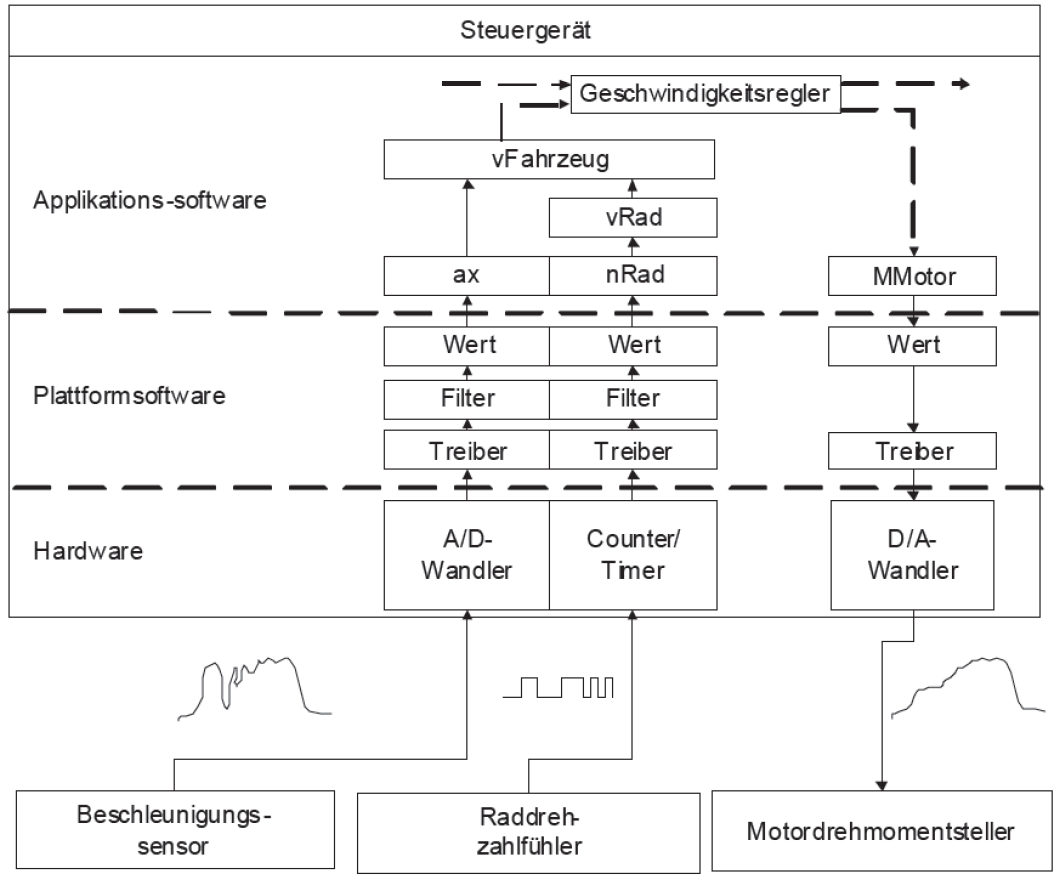
\includegraphics[width=0.8\columnwidth]{images/embedded_system_aufbau_schichten.png}
\end{center}


\subsection{Beispiele}

\vspace{-0.2cm}

\begin{minipage}[t]{0.48\columnwidth}
    \raggedright
    \subsubsection*{Fahrrad-Computer}

    \begin{outline}
        \1 GPS-Navigation
        \1 Geschwindigkeits- und Trittfrequenzmessung
        \1 Pulsmesser
        \1 Drahtlosübertragung (ANT+)
        \1 Interface zu elektronischer Gangschaltung
        \1 Barometer, Thermometer
        \1 Trainingsassistent
        \1 Display
    \end{outline}

    \subsubsection*{Weitere Beispiele}

    \begin{itemize}
        \item Smartphone
        \item Mobile Base Station
        \item CNC-Bearbeitungszentdrum
        % \item Schubumkehr bei Flugzeugen
        % \item Lungenzustandsdetektion mit Elektro-Impedanztomographie (EIT)
        \item Hörgerät
    \end{itemize}
\end{minipage}
\hfill
\begin{minipage}[t]{0.48\columnwidth}
    \raggedright
    \subsubsection*{Auto}

    \begin{outline}
        \1 Sicherheitsrelevante Aufgaben
            \2 ABS, ASR
            \2 Motorenregelung
            \2 Drive-by-wire
            \2 Autonom fahrende Autos
        \1 Unterhaltung / Komfort
            \2 Radio / CD / etc.
            \2 Navigation
            \2 Klima
        \1 Mehrere Netzwerke
            \2 CAN, LIN, Ethernet
        \1 Echtzeitteile und andere
        \1 Von einfachsten $\micro$Cs bis DSPs und GPUs 
    \end{outline}

    \textrightarrow\ Auto ist ein riesiges Embedded System
\end{minipage}


\subsection{Deeply Embedded System}

\begin{itemize}
    \item 'Einfaches' Embedded System, mit \textbf{minimaler Benutzerschnittstelle}, üblicherweise mit \textbf{keinerlei GUI}
        und \textbf{ohne Betriebssystem}
    \item Beschränkt auf \textbf{eine} Aufgabe (z.B. Regelung eines physikalischen Prozesses)
    \item Muss oft zeitliche Bedingungen erfüllen \textrightarrow\ Echtzeitsystem
\end{itemize}


\subsubsection{Beispiele -- Deeply Embedded System}

\begin{minipage}[t]{0.3\columnwidth}
    \begin{itemize}
        \item Hörgerät
        \item Motorenregelung
    \end{itemize}
\end{minipage}
\hfill
\begin{minipage}[t]{0.3\columnwidth}
    \begin{itemize}
        \item ABS-Controller
        \item 'Sensor' im IoT
    \end{itemize}
\end{minipage}
\hfill
\begin{minipage}[t]{0.3\columnwidth}
    \begin{itemize}
        \item etc...
    \end{itemize}
\end{minipage}


\subsection{Betriebssysteme bei Embedded Systems}

\begin{outline}
    \1 Es kommen Betriebssysteme wie (Embedded) Linux oder Android zum Einsatz \\
        \textrightarrow\ \textbf{Achtung: Linux und Android sind nicht echtzeitfähig!}
    \1 Wenn Echtzeit verlangt wird: real-time operating systems (RTOS)
        \2 Beispiele: Zephyr, Free RTOS (Amazon), TI-RTOS (Texas Instuments), etc. \\
            \textrightarrow\ RTOS siehe Abschnitt \ref{Real-Time Operating Systems (RTOS)}
\end{outline}


\subsection{Bare Metal Embedded System}

\begin{itemize}
    \item Es kommt \textbf{keinerlei Betriebssystem} zum Einsatz
    \item Bare Metal Embedded Systems sind recht \textbf{häufig}, insbesondere bei \textbf{Deeply Embedded Systems}
    \item Bare Metal Embedded Systems stellen besondere Ansprüche an Programmierung
\end{itemize}


\subsection{Zuverlässigkeit}

\begin{minipage}[c]{0.45\columnwidth}
    \pgfplotsset{samples=100}   % sample points to make graph smooth

\begin{center}
    \begin{tikzpicture}
        [
            scale = 0.6,
            >=latex
        ]
        \begin{axis}
            [
                title=\textbf{Zuverlässigkeit},
                width=8cm,
                height=5cm,
                xmin=-0.2, xmax=8, ymin=-0.1, ymax=1.3, axis lines=middle,
                x label style={at={(axis description cs:0.5,0)},anchor=north},
                y label style={at={(axis description cs:-0.1,0.5)},rotate=90,anchor=south},
                xlabel=Zeit,
                ylabel=Wahrscheinlichkeit,
                xtick=\empty,
                ytick={0, 0.2, 0.4, 0.6, 0.8, 1, 1.2}
                %grid
            ]
        
            % plot
            \addplot[color=blue, thick, domain=-0:10]{exp(-0.5*x)};
        \end{axis}
        
    \end{tikzpicture}
\end{center}
\end{minipage}
\hfill
\begin{minipage}[c]{0.5\columnwidth}
    \raggedright

    \begin{itemize}
        \item Je länger das System läuft, desto weniger zuverlässig ist es
        \item Die Wahrscheinlichkeit für einen Ausfall steigt stetig
    \end{itemize}
    
    \vspace{0.2cm}

    \textbf{Achtung:} Hier ist nur die Alterung der Hardware berücksichtigt
\end{minipage}


\subsection{Verfügbarkeit}

Die Verfügbarkeit A (availability) ist der Anteil der Betriebsdauer innerhalb dessen das System seine Funktion erfüllt.
$$ \text{Verfügbarkeit} = \frac{\text{Gesamtzeit} - \text{Ausfallzeit}}{\text{Gesamtzeit}} $$


% \subsection{Abstraktionsschichten}

% \begin{itemize}
%     \item Bei $\micro$C-Programmierung (Firmware) müssen oft Bitmuster in Register geschrieben werden
%     \item Solche Register-Zugriffe dürfen \textbf{nicht} 'willkürlich' überall im Code erfolgen \\
%         \textrightarrow\ schlecht lesbar, schlecht portiertbar, fehleranfällig
%     \item \textbf{Damit Code lesbarer und besser auf andere Platform portierbar wird, beinhaltet jeder professionelle Code einen
%         Hardware Abstraction Layer (HAL)}
%     \item HAL führt \textbf{nicht} zum Verlust bei Laufzeit, wenn korrekt implementiert
% \end{itemize}


% \subsubsection{Hardware-abstraction-layer (HAL)}

% \begin{itemize}
%     \item Trennt HW-Implementierung von SW-Logik
%     \item Gleiche SW kann auf verschiedene HW verwendet werden \textrightarrow\ Portabilität
%     \item HW-Komponenten können einfach ausgetauscht werden \textrightarrow\ Flexibilität
% \end{itemize}


        % Modellierung von Embedded (real-time) Systems (Model Driven Development, MDD)
        \section{Real-Time System (Echtzeitsystem)}

\subsection{Definitionen}

\subsubsection{Real-Time System (Echtzeitsystem)}

\begin{itemize}
    \item Ein Echtzeitsystem ist ein System, das Informationen \textbf{innerhalb einer definierten Zeit (deadline) bearbeiten} muss. \\
        \textrightarrow\ Explizite Anforderungen an \textbf{turnaround-time} (Antwortzeit) müssen erfüllt sein
    \item Wenn diese Zeit nicht eingehalten werden kann, ist mit einer \textbf{Fehlfunktion} zu rechnen.
\end{itemize}

\vspace{0.2cm}

\begin{minipage}[t]{0.55\columnwidth}
    \begin{center}
        \myul{\textbf{Typisches Echtzeitsystem}}

        \vspace{0.1cm}

        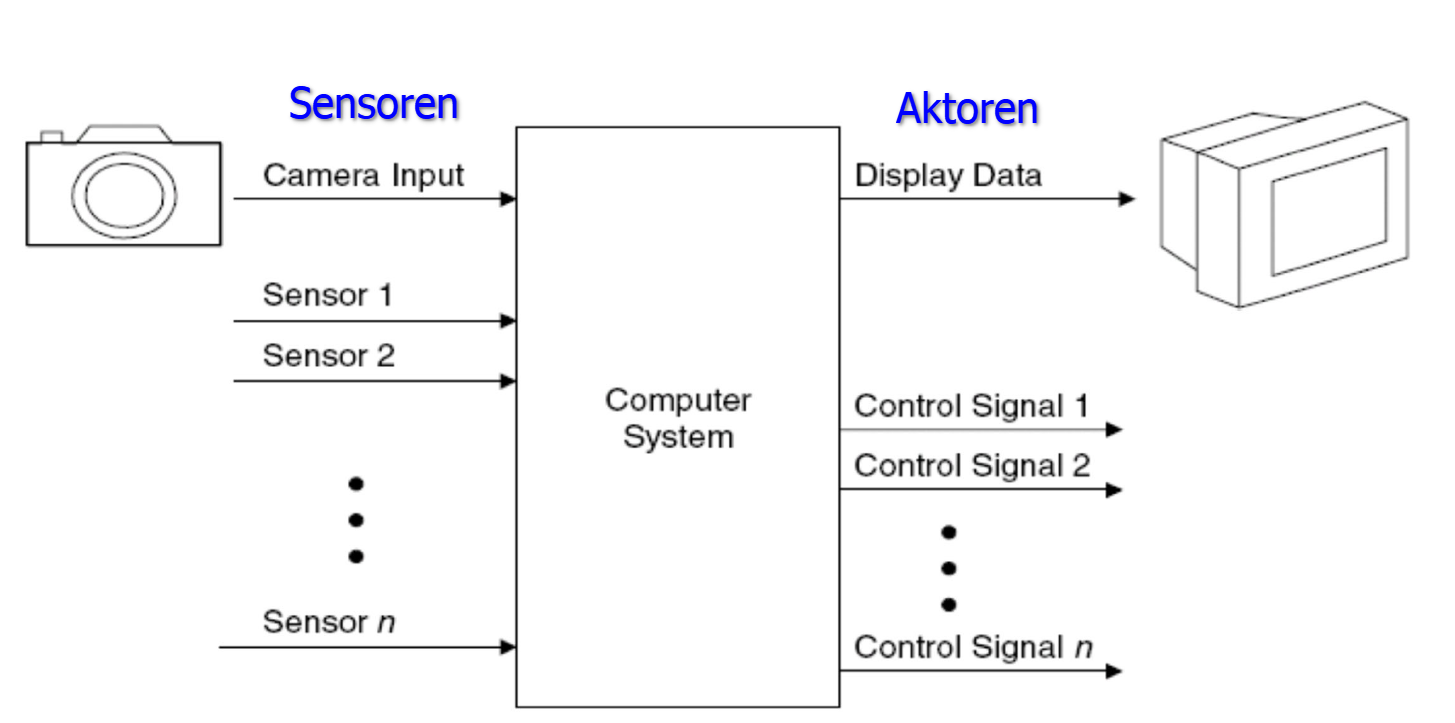
\includegraphics[width=\columnwidth]{images/typisches_echtzeitsystem.png}
    \end{center}
\end{minipage}
\hfill
\begin{minipage}[t]{0.4\columnwidth}
    \begin{center}
        \myul{\textbf{Repräsentation RT-System}}

        \vspace{0.1cm}

        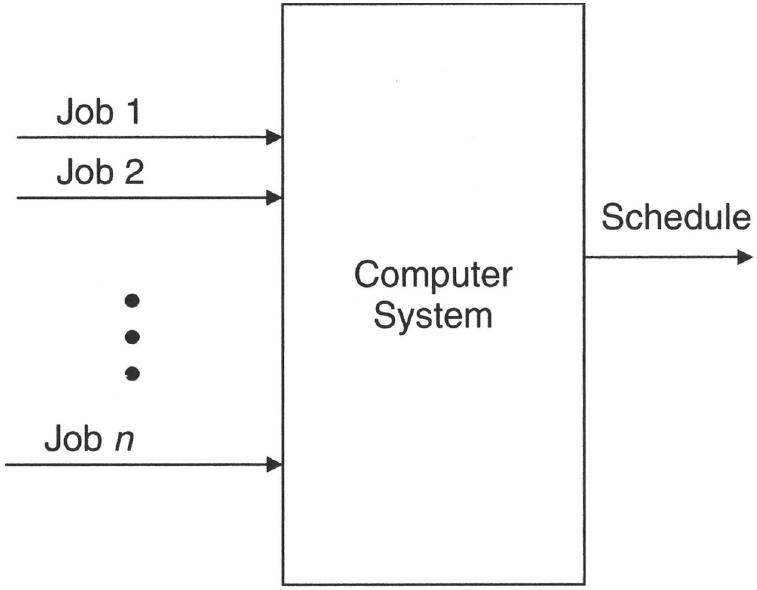
\includegraphics[width=0.7\columnwidth]{images/typische_repraesentation_echtzeitsystem.png}

        Sequenz von Aufgaben (Jobs) müssen zeitlich geplant (scheduled) werden
    \end{center}
\end{minipage}



\subsubsection{Zeitdefinitionen (Task)}

\begin{center}
    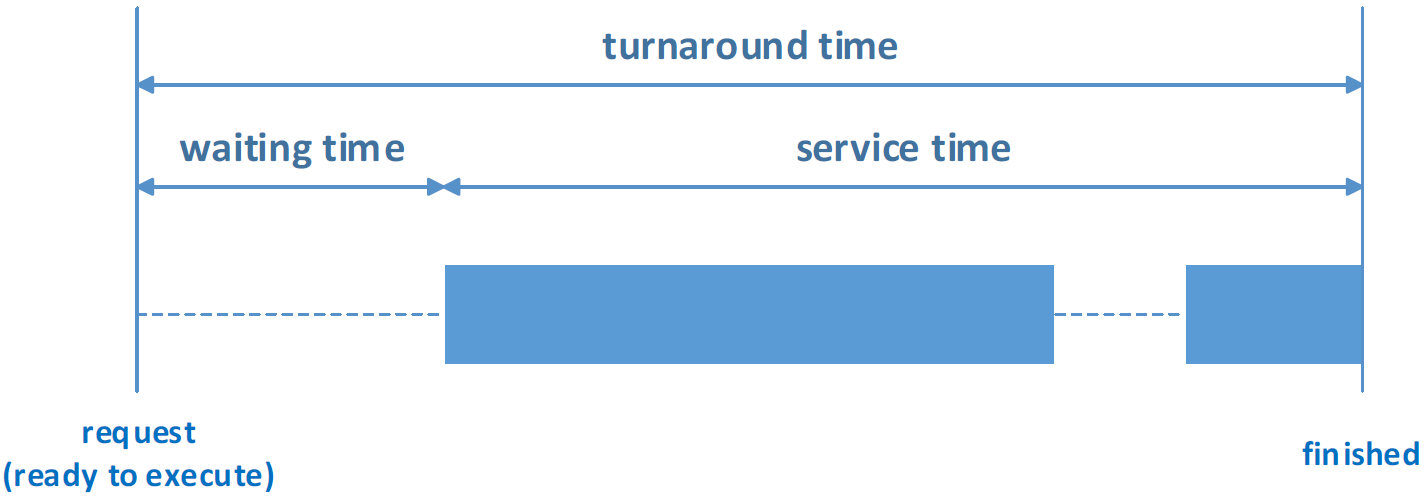
\includegraphics[width=0.7\columnwidth]{images/zeitdefinitionen_task.png}
\end{center}

\begin{outline}
    \1 \textbf{turnaround time:} (response time, Antwortzeit) 
        \2 Startet, wenn der Task bereit zur Ausführung ist und endet, wenn der Task fertig abgearbeitet ist
        \2 Zeit zwischen dem Vorhandensein von Eingangswerten an das System (Stimulus) bis zum Erscheinen der gewünschten Ausgangswerte.
    \1 \textbf{waiting time:} (Wartezeit)
        \2 Zeit zwischen Anliegen der Eingangswert und Beginn der Abarbeitung des Tasks
    \1 \textbf{service time:} (Bearbeitungszeit)
        \2 Zeit für Abarbeitung des Tasks \textrightarrow\ Unterbrechungen bzw. (preemptions) möglich 
\end{outline}


\subsection{Fehlverhalten eines Systems (failed system)}

\begin{itemize}
    \item Ein fehlerhaftes System (failed system = missglücktes System) ist ein System, das nicht alle formal
        definierten Systemspezifikationen erfüllt.
    \item \textbf{Die Korrektheit eines RT Systems bedingt sowohl die Korrektheit der Outputs als auch die Einhaltung
        der zeitlichen Anforderungen.}
\end{itemize}


\subsection{Echtzeitdefinition -- Verschiedene Echtzeitsysteme}

\begin{outline}
    \1 \textbf{soft real-time system} (weiches Echtzeitsystem)
        \2 Durch Verletzung der Antwortzeiten wird das System \textbf{nicht} ernsthaft beeinflusst
        \2 Es kommt zu Komforteinbussen
    \1 \textbf{hard real-time system} (hartes Echtzeitsystem)
        \2 Durch Verletzung der Antwortzeiten wird das \textbf{System ernsthaft beeinflusst}
        \2 Es kann zu einem kompletten Ausfall oder katastrophalem Fehlverhalten kommen
    \1 \textbf{firm real-time system} (festes Echtzeitsystem)
        \2 Kombination aus soft real-time system und hard real-time system
        \2 Durch Verletzung einiger weniger Antwortzeiten wird das System nicht ernsthaft beeinflusst
        \2 Bei vielen Verletzungen der Antwortzeiten kann es zu einem kompletten Ausfall oder katastrophalem Fehlverhalten kommen
\end{outline}


\subsubsection{Beispiele verscheidener Echtzeitsysteme}

\begin{center}
    \begin{tabular}{@{}lll@{}}
        \toprule
        \textbf{System}     & \textbf{Klassifizierung}  & \textbf{Erlärung}                             \\
        \midrule
        Geldautomat         & soft                      & Auch wenn mehrere Deadlines nicht eingehalten \\
                            &                           & werden können, entsteht dadurch keine         \\
                            &                           & Katastrophe. Im schlimmsten Fall erhält ein   \\
                            &                           & Kunde sein Geld nicht.                        \\
        \midrule
        GPS-gesteuerter     & firm                      & Wenn die Positionsbestimmung versagt, könnte  \\
        Rasenmäher          &                           & das Blumenbeet der Nachbarn platt gemäht      \\
                            &                           & werden.                                       \\
        \midrule
        Regelung eines      & hard                      & Das Versagen der Regelung kann dazu führen,   \\
        Quadrocopters       &                           & dass der Quadrocopter ausser Kontrolle        \\
                            &                           & gerät und abstürzt.                           \\
        \bottomrule
    \end{tabular}
\end{center}


% \subsection{Determinsismus (determinacy)}


% \subsection{Auslastung (utilization)}


% \subsection{Real-time Scheduling}

        % Hardware/Software Codesign
        % Finite State Machines (Anwendung, Implementationen in C und C++)
        % Gleichzeitigkeit (Concurrency)
        % POSIX-Programmierung
        % Event-based Systems
        % Embedded Software Patterns
        % Multicore Systems mit Multistage-Caches, Interprozesskommunikation, Shared Memory
        % Real-time Operating System (RTOS)
        % Hardware Abstraction Layer (HAL) in C und C++
    \end{layout}
\end{document}
